\documentclass{article}

% Document Packages
\usepackage{hyperref}
\hypersetup{
    colorlinks=true,
    linkcolor=blue,
    filecolor=magenta,
    urlcolor=cyan,
}
\usepackage{geometry}
\geometry{
	a4paper,
	noheadfoot=true,
	left=1.0in,
	right=1.0in,
	top=1.0in,
	bottom=1.0in,
}

% Tikz and Figure Packages
\usepackage{caption}
\usepackage{amsmath} % aligned env
\usepackage{tikz}

\usetikzlibrary{decorations.pathreplacing}

%%%%%%%%%%%%%%%%%%%%%%%%%%%%%%%%%%%%%%%%%%%%%%%%%%%%%%%%%%%
%%% Titles
%%%%%%%%%%%%%%%%%%%%%%%%%%%%%%%%%%%%%%%%%%%%%%%%%%%%%%%%%%%

\title{Latex Tikz Examples\\Model Timeline with Dynamically Sized Panes and Text Blocks \\ Eight Dynamic Panes and Four Dynamic Text Blocks}
\author{\href{https://fanwangecon.github.io/}{Fan Wang}\thanks{https://fanwangecon.github.io, repository: \href{https://fanwangecon.github.io/Tex4Econ/}{Tex4Econ}}}
\date{\today}

%%%%%%%%%%%%%%%%%%%%%%%%%%%%%%%%%%%%%%%%%%%%%%%%%%%%%%%%%%%
%%% Define Core Frame
%%%%%%%%%%%%%%%%%%%%%%%%%%%%%%%%%%%%%%%%%%%%%%%%%%%%%%%%%%%

\newcommand{\tikzframeeight}[7]{

  %%% 1. Define Figure Width and Height as Ratio of Page Width and Height
  % param 7 rescales, set same as every node/.style={scale=#7}
  \def\fgiw{#1*\textwidth*#7}  
  \def\fgih{#2*\textheight*#7}

  %%% 2. Cut Figure into Four Quadrants
  % fgiwm: breaks the left and right quadrants
  % fgihm: breaks the top and bottom quadrants
  \def\fgiwm{#3*\fgiw}
  \def\fgihm{#4*\fgih}

  %%% 3. Divide each quadrant into two parts, 8 parts
  % each quadrant now has small left edge or small right edge
  % fgile: break a small piece off left quadrant
  % fgire: break a small piece off left quadrant
  \def\fgile{#5*\fgiw}
  \def\fgire{#6*\fgiw}

  %%% Commonly Used Non-Parameters
  % left pane horizontal middle point, align horizontally middle pane
  \def\fgiwlm{\fgile*0.5 + \fgiwm*0.5}
  % right pane horizontal middle point, align horizontally middle in pane
  \def\fgiwrm{\fgiwm*0.5 + \fgire*0.5}

  % fgihtb: figure internal height top pane bottom
  % vertically bottom 10 percent space of top pane space
  \def\fgihtb{\fgihm + \fgih*0.085 - \fgihm*0.085}

  % fgihtm: figure internal height top and bottom pane middle height
  % top panel vertical middle spot, align vertically center
  \def\fgihtm{\fgihm*0.5 + \fgih*0.5}
  % bottom panel vertical middle spot, align vertically center
  \def\fgihbm{\fgihm*0.5}


  % There is a flow line on top, limited text
  % three parts, left prior, right after, middle current.
  % current in two parts, shock realization and choices.
  % In top part, span charts, simple text
  % in bottom part, sufficient height to allow for detailed text
  % descriptions.

  % Bottom and top lines
  \draw [dotted] (0, \fgih) -- (\fgiw, \fgih);
  \draw [dotted] (0, 0    ) -- (\fgiw, 0    );

  % Left and right lines
  \draw [dotted] (0,     0) -- (0,     \fgih);
  \draw [dotted] (\fgiw, 0) -- (\fgiw, \fgih);

  % verticle middle line
  \draw [dotted] (\fgiwm, 0) -- (\fgiwm,   \fgih);
  % horizontal middle line (divide text and flow)
  \draw [solid] (0, \fgihm) -- (\fgiw,   \fgihm);

  % left border last period
  \draw[dashed] (\fgile, 0  ) -- (\fgile,   \fgih);
  % right border next period
  \draw[dashed] (\fgire, 0  ) -- (\fgire,   \fgih);

  % Heading for the left-most, right-most and center areas
  \node[align=center] at (0.5*\fgile,             0.900*\fgih) {last\\period};
  \node[align=center] at (0.5*\fgiw,              0.900*\fgih) {current period};
  \node[align=center] at (0.5*\fgire + 0.5*\fgiw, 0.900*\fgih) {next\\period};

  % Sub-label for the left and right part of center pane 
  \node[align=center] at (\fgiwlm, \fgihtb) {shocks};
  \node[align=center] at (\fgiwrm, \fgihtb) {asset choices};

  % Arrows in top pane, between left border center, center left and right and center to right border
  \draw [->, line width=0.25mm] (\fgile-0.2*\fgile, \fgihtm) -- (\fgile+0.2*\fgile, \fgihtm);
  \draw [->, line width=0.25mm] (\fgiwm-0.2*\fgile, \fgihtm) -- (\fgiwm+0.2*\fgile, \fgihtm);
  \draw [->, line width=0.25mm] (\fgire-0.2*\fgile, \fgihtm) -- (\fgire+0.2*\fgile, \fgihtm);
}

%%%%%%%%%%%%%%%%%%%%%%%%%%%%%%%%%%%%%%%%%%%%%%%%%%%%%%%%%%%
%%% Define text block
%%%%%%%%%%%%%%%%%%%%%%%%%%%%%%%%%%%%%%%%%%%%%%%%%%%%%%%%%%%

\newcommand{\textA}{choose \\ $k, b$}
\newcommand{\textB}{$\Gamma\left(k,b,\epsilon\right)$}
\newcommand{\textC}{$\begin{aligned}c &= \Gamma\cdot\phi\\k &= \Gamma\cdot\phi\cdot\theta\\b &= \Gamma\cdot\phi\cdot\left(1-\theta\right)\end{aligned}$}
\newcommand{\textD}{draw \\$\epsilon^{\prime}$ shock}

\newcommand{\tikztextblock}[4]{
% #1=choose \\ $k, b$ 
% #2=$\Gamma\left(k,b,\epsilon\right)$
% #3=$\begin{aligned}c &= \Gamma\cdot\phi\\k &= \Gamma\cdot\phi\cdot\theta\\b &= \Gamma\cdot\phi\cdot\left(1-\theta\right)\end{aligned}$
% #4=draw \\$\epsilon^{\prime}$ shock
% 2. Text
\node[align=center] (A) at (0.5*\fgile, \fgihtm)
{#1};
\node[align=center] (B) at (\fgiwlm, \fgihbm)
{#2};
\node[align=center] (C) at (\fgiwrm, \fgihbm)
{#3};
\node[align=center] (D) at (0.5*\fgire + 0.5*\fgiw, \fgihtm)
{#4};
}

\begin{document}

\maketitle

Generate a eight pane model timeline tikz structure. The proportional sizes of each pane is determined by parameters, and are porportional to pages. The 8 pane tables have 7 parameters that auto shift the figures.


\section{Empty Frames with Eight Panes}
The idea is that the top panes would show overall model timeline. The bottomw below horizontal line spaces could have equations that provide more information sufficiently about what is happening in timeline above. 
\begin{center}
  \begin{tikzpicture}[scale=1.0, every node/.style={scale=1.0}]
    \tikzframeeight{1}{0.25}{0.5}{0.35}{0.125}{0.875}{1.0}
  \end{tikzpicture}
\end{center}
\begin{center}
  \begin{tikzpicture}[scale=1.0, every node/.style={scale=0.5}]
    \tikzframeeight{1}{0.25}{0.6}{0.35}{0.125}{0.875}{0.5}
  \end{tikzpicture}
\end{center}
\begin{center}
  \begin{tikzpicture}[scale=1.0, every node/.style={scale=0.75}]
    \tikzframeeight{1}{0.20}{0.2}{0.50}{0.125}{0.875}{0.75}
  \end{tikzpicture}
\end{center}
\pagebreak

\section{Eight Dynamic Panes and Four Dynamic Text Blocks}

Now in addition to the frame structure, add in text, the texts are dynamically controlled with textblocks. The positions are dynamically sized automatically. Text contents could change. 

\begin{center}
  \begin{tikzpicture}[scale=1.0, every node/.style={scale=1.0}]
    \tikzframeeight{1}{0.25}{0.5}{0.35}{0.125}{0.875}{1.0}
    \tikztextblock{\textA}{\textB}{\textC}{\textD}    
  \end{tikzpicture}
\end{center}
\begin{center}
  \begin{tikzpicture}[scale=1.0, every node/.style={scale=0.5}]
    \tikzframeeight{1}{0.25}{0.6}{0.35}{0.125}{0.875}{0.5}
    \tikztextblock{hello \\ there}{block two}{this is third}{now \\ fourth \\ text \\ block}
  \end{tikzpicture}
\end{center}
\begin{center}
  \begin{tikzpicture}[scale=1.0, every node/.style={scale=0.75}]
    \tikzframeeight{1}{0.20}{0.2}{0.50}{0.125}{0.875}{0.75}
    \tikztextblock{$k$}{$\Gamma$}{$\Lambda$ \\ here you go \\ yes works}{$\epsilon$}
  \end{tikzpicture}
\end{center}

\end{document}
